\chapter{绪论}
\section{研究背景}
随着计算机视觉(Computer Vision)
和自然语言处理(Natural Language Processing)技术的迅猛发展,
跨模态智能理解成为人工智能研究的重要方向之一。
其中,视觉问答(Visual Question Answering, VQA)\cite{goyal2017making}任务因其广泛的应用前景和挑战性,
受到了学术界和工业界的广泛关注。

视觉问答是一种多模态任务,它要求计算机能够基于给定的图像内容,
理解并回答关于该图像的自然语言问题。例如,给定一幅包含动物的图片,
系统需要能够回答“这只动物是什么颜色?”或“图片中有几只猫?”等问题。
这一任务的核心在于多模态信息的深度融合,即如何在视觉特征和语言信息之间建立有效的联系。

视觉语言模型(Visual Language Model, VLM)是一种多模态模型,能够同时处理图像和文本信息,并生成与图像内容相关的自然语言响应。
如图\ref{fig:vlm-example}所示为VLM的一个简单流程示例。
VLM通过将视觉编码器与大语言模型结合,赋予模型“看”与“理解”的能力。与传统的计算机视觉模型不同,VLM 不受固定
类别集或特定任务 (如分类或检测) 约束。在大量文本和图像/视频字幕对的语料上进行重新训练,
VLM 可以用自然语言进行指导,并用于处理许多典型的视觉任务以及新的生成式 AI 任务,
例如摘要和视觉问答。如图\ref{fig:vlm-architecture}所示为VLM的通用架构,包括视觉编码器、投影器和大语言模型(Large Language Model, LLM)三个部分。
视觉编码器(如CLIP模型)具有图像与文本的关联能力,负责提取图像特征。投影器由一组网络层构成,负责将视觉特征转换为LLM可理解的标记(Token)。
LLM负责生成文本输出,支持对话、推理等任务,目前任何现有的LLM(如ChatGPT、Llama、DeepSeek等)都可以用来构建VLM。
\begin{figure}
    \centering
    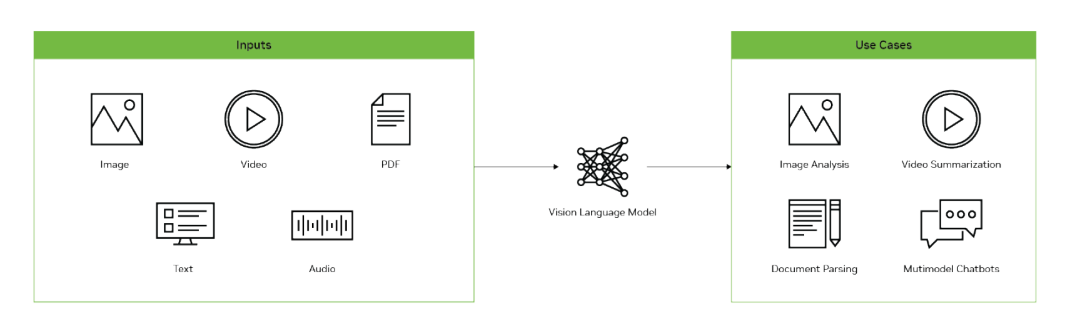
\includegraphics[width=\textwidth]{figures/VLM-example.png}
    \caption{视觉语言模型用例}
    \label{fig:vlm-example}
\end{figure}

\begin{figure}[htb]
    \centering
    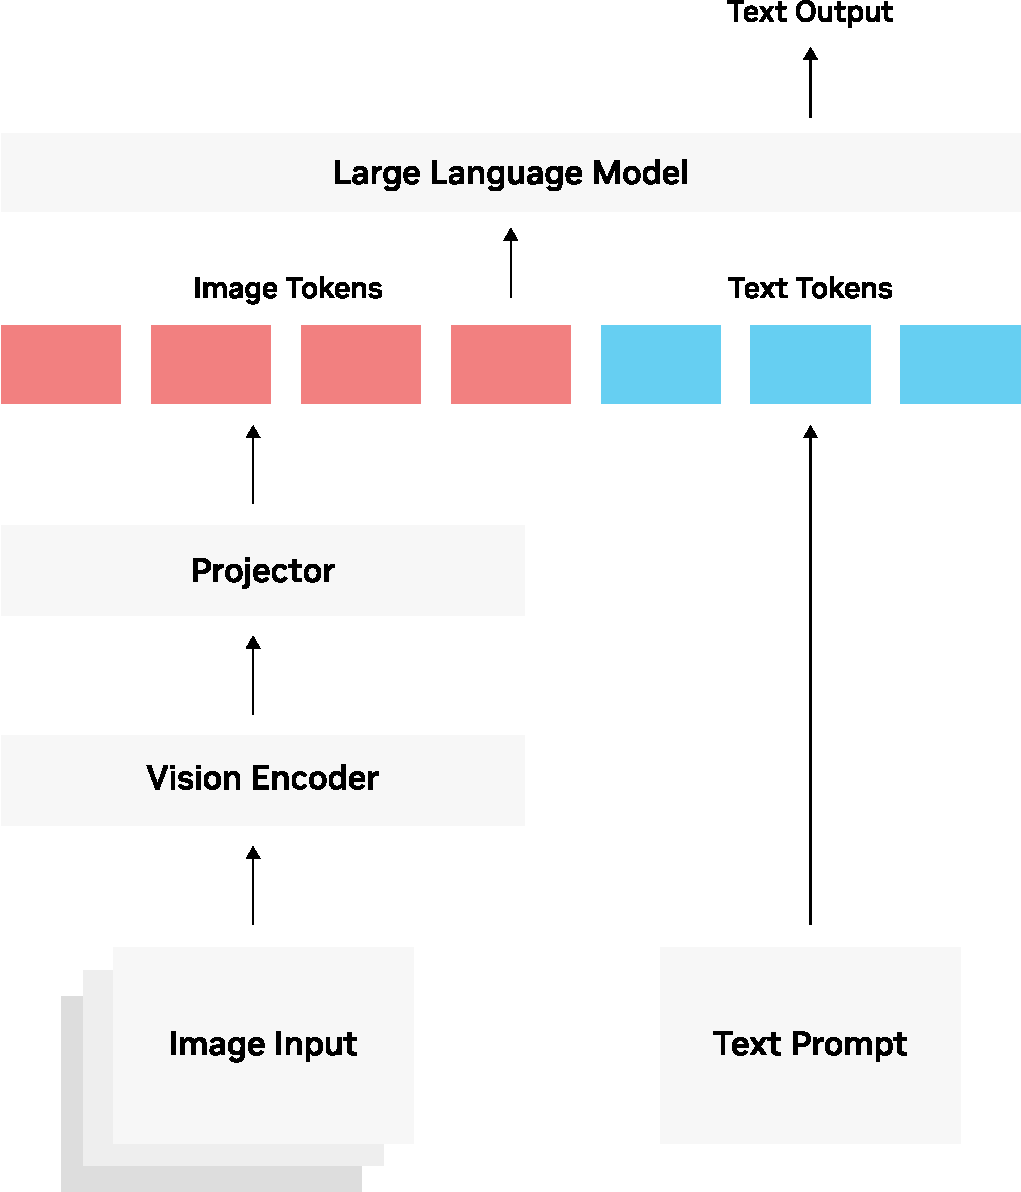
\includegraphics[scale=0.6]{figures/vlm-architecture-diagram-crop.pdf}
    \caption{视觉语言模型的通用三部分架构}
    \label{fig:vlm-architecture}
\end{figure}

尽管VLM在图像分类\cite{pratt2023does}、字幕生成\cite{alaluf2024myvlm}、
目标检测\cite{kuo2022f}、视频理解\cite{huang2024lita}和文档解析\cite{lv2023kosmos}
等各种任务中取得了良好效果,但这些模型在空间推理方面
仍然面临重大挑战。具体表现为难以区分"左"和"右"、"上"和"下"等简单空间概念,以及"前"与"后"、"内"与"外"、"近"与"远"等复杂空间关系\cite{fu2024blink}\cite{majumdar2024openeqa}\cite{zhang2024countercurate}。
此外,VLM在处理细节模糊或者部分遮挡的场景时,其表现类似于视力不佳的人,难以捕捉到图像中的细节信息,从而影响
其问答或者描述的准确性,这表明目前VLM对处理部分可见场景的问题仍有很大的局限性\cite{rahmanzadehgervi2025visionlanguagemodelsblind}。
正确理解并推理空间关系的能力,不仅对视觉理解至关重要,而且对智能机器人\cite{gao2024physically}\cite{nasiriany2024pivot}
和增强现实\cite{konenkov2024vr}等领域的现实应用也至关重要。
在这些领域中,精确的空间感知能力对于导航\cite{huang2023visual}、物体操控\cite{gao2024physically}
和与现实世界的交互\cite{driess2023palm}等任务至关重要。
在自动规划课程教学中,需要使用智能机器人为学生进行操纵物块、绕避障碍物等动作的演示。
而实际场景中,机器人可能会因为物体遮挡而无法直接看到目标物体的位置,进而需要结合已知信息进行推理,
这就要求机器人的空间推理系统在部分可见的场景下具备推理能力,像人类一样根据周围环境信息和已有先验知识,做出正确的决策。
因此,对多模态模型的空间推理能力展开研究,增强其对部分可见场景问题的推理能力,具有十分重要的现实意义和应用价值。

为了解决多模态模型在空间推理方面的问题,研究者们提出了一些新的方法。近年来,
神经符号方法(Neuro-Symbolic Methods)得到了广泛关注。在多模态空间推理场景中,
神经符号方法使用深度学习技术进行感知,为输入的图像和问题分别生成符号表示,再使用符号系统进行推理求解,
可以有效提升多模态模型在空间推理方面的能力。

在神经符号方法中,神经网络的选择十分多样,通常包括卷积神经网络(Convolution Neural Network, CNN)、
循环神经网络(Recurrent Neural Network, RNN)及其变体、图神经网络(Graph Neural Network, GNN)和
Transformer架构及LLM。相比其它神经网络,LLM用于神经符号系统,具有以下突出优势:
\begin{enumerate}[itemsep=0pt,parsep=0pt]
    \item 丰富的预训练知识库。LLM在大规模语料上进行预训练,具备广泛的世界知识和语言理解能力,这使得它们在处理涉及常识推理和多领域知识整合时,比专门针对单一任务训练的网络更具优势。
    \item 自然语言理解与生成能力。LLM能够将符号系统产生的抽象逻辑或规则,用自然语言进行解释和反馈,从而降低了人机交互的门槛,并使得系统的推理过程更易于理解和验证。
    \item 零样本/少样本学习能力。由于在大规模数据上学习到了通用的语言模式,LLM在面对新领域或数据较少的任务时,往往能够直接发挥作用,从而提高神经符号系统的泛化能力。
    \item 灵活的上下文建模。LLM能够捕捉长距离依赖和上下文信息,这对于将符号系统中离散的知识点进行有机整合,以及在复杂场景中实现动态推理具有重要意义。
\end{enumerate}
结合以上各项理由,将LLM作为神经符号系统中的神经模块,能够与符号系统形成互补,既利用符号逻辑的严谨性,又发挥神经网络在语义理解和自然语言生成方面的优势,从而构建更强大、更灵活的智能系统。

在神经符号方法中,符号系统的选择同样多种多样,例如知识图谱嵌入(Knowledge Graph Embeddings, KGE)、逻辑神经网络(Logical
 Neural Networks, LNN)都为信息表示和推理提供了新思路。然而,在当前的研究和应用中,回答集编程(Answer Set Programming,ASP)往往被更多
地采用作为符号系统。ASP是一种声明式编程范式,可用于解决复杂的人工智能问题,其起源于对逻辑编程、非单调推理和知识表示的研究。
相比其它符号系统,ASP被更多用于神经符号方法中,主要是由于以下几点优势:(1)明确的逻辑语义与可解释性。ASP基于严格定义的逻辑规则,其推理过程透明、易于解释。这一特性在需要精确推理和结果可验证的任务中尤为重要\cite{gelfond1988stable};
(2)强大的非单调推理能力。ASP自然支持非单调逻辑推理,能够处理默认情况和异常情形,这使其在面对现实世界中不完全或动态变化的信息时表现出色\cite{gelfond1988stable};
(3)成熟的求解器与工具支持。像Clingo这样的ASP求解器已经经过长期验证,具有高效、稳定的特点,能够处理大规模问题,这为实际应用提供了有力保障\cite{gebser2012answer};
(4)便于与神经网络等模块整合。ASP的声明式表达方式使其易于与神经网络输出的信息对接,形成互补优势,从而提升整体系统的推理能力\cite{garcez2002neural}。
ASP的这些特性使得它作为符号系统的杰出代表,被广泛应用于神经符号方法中。

尽管神经网络采用了预训练的LLM,而符号系统部分选用了ASP,但将二者有效结合在一起仍然是一项复杂的任务。
为此,近年来出现了一些神经符号框架,试图通过模块化设计和统一接口来简化LLM与ASP的集成开发流程\cite{wang2024dspybasedneuralsymbolicpipelineenhance}。
尽管现有的框架为LLM结合ASP的开发过程提供了诸多便利,降低了使用门槛,然而其在ASP规则的自动拓展方面存在不足,
需要依赖人工干预进行规则扩充,在这一方面仍存在改进空间。

为了测试模型解决空间推理问题的能力,涌现了诸如CLEVR、GQA、COCO等数据集。
这些数据集由问题答案对(Question and Answer Pair,以下简称QA对)组成,
并且包含问题对应的场景图像。其中,CLEVR数据集因高度结构化的场景构造、精确标注的物体属性及复杂的空间关系,而被广泛用于检测智能机器人的环境感知模块在空间推理方面的能力。
然而,CLEVR数据集的图像均是基于完整场景生成,所有回答问题的信息在对应的图像中都直接可见,
缺乏现实环境中常见的部分可见性的情形,不能有效考察模型解决部分可见场景问题的能力\cite{sam-abraham-etal-2024-clevr}。

基于上述背景,本文重点关注提升视觉问答系统对部分可见场景问题的推理能力,
并对CLEVR数据集进行改进,以对使用神经符号方法的视觉问答系统回答该类问题的能力进行定量评估。
\section{相关研究现状}
基于以上背景,本节主要从视觉问答的发展与现状、空间推理的发展与现状、
视觉问答数据集的发展与现状、生成ASP程序的发展与现状、神经符号方法在空间推理中的发展与现状来进行综述。

\subsection{视觉问答的发展与现状}
VQA任务最早由Antol\cite{Antol2015VQA}等人在2015年提出,标志着VQA研究早期阶段的开始。这一阶段的VQA系统采用比较简单的架构,主要包括视觉编码器、语言编码器和融合模块。
Ren\cite{ren2015exploring}等人将采用预训练的卷积神经网络(Convolutional Neural Network, CNN)作为视觉编码器提取图像特征,采用循环神经网络(Recurrent Neural Network, RNN)作为语言编码器或
提取问题特征。Malinowski\cite{malinowski2015neural}等人在视觉编码器上同样采用CNN,在语言编码器上则是采用长短期记忆(Long Short-Term Memory , LSTM)来生成问题的答案。
融合模块通常采用简单的拼接或注意力机制融合视觉和语言特征。这些系统在一些简单的VQA数据集上取得了不错的性能,但在处理复杂的空间推理问题时表现较差。

随着计算机视觉和自然语言处理技术的发展,VQA系统逐步引入了更高级的特征提取与融合方法。
例如,Yao\cite{lu2019look}等人将区域提议网络(RPN)引入到VQA模型中,以增强对图像中物体的感知能力。
注意力机制也逐渐引入VQA模型中,例如Xu\cite{xu2016stacked}等人提出堆叠注意力网络(SANs),
通过多层次注意力机制,逐步聚焦于图像和问题的关键部分,从而提升了VQA模型的推理能力。

在2019年前后,得益于基于Transformer的预训练语言模型的兴起,VQA研究取得了显著进展。如BERT、ViLBERT和LXMERT等模型通过联合训练大规模的视觉和语言数据,
学得如何在同一嵌入空间中表示视觉和文本信息,极大程度上提升了VQA的准确性和鲁棒性。
例如,Tan\cite{Tan2019LXMERT}等人提出了LXMERT模型,将预训练的BERT模型与视觉编码器相结合,实现了对图像和问题的联合编码。

如今,VQA的研究已经进入了全新阶段。随着大规模视觉语言模型(如GLIP、GPT-4等)的应用,VQA模型已经能够处理更加复杂的任务,不仅处理特定问题时效果出色,而且可以进行
跨模态推理,通过多种信息源之间的互动生成更加丰富和精准的答案。OpenAI的研究团队\cite{radford2021learning}在CLIP模型中,应用了自监督学习的方法
,利用海量的图文对数据进行训练,实现了视觉和语言的统一表示,且训练过程无需人工标注,充分体现了自监督学习的优势。Salesforce的研究团队\cite{li2022blip}在BLIP模型中,
通过生成式预训练任务,提升了视觉语言模型在理解和生成方面的性能。

\subsection{空间推理的研究现状}
近年来,研究人员在利用LLM进行空间推理方面取得了显著进展。Hong\cite{hong20233d}等人将重点放在
从多视角图像重建场景,例如通过点云或神经场构建三维表示,并结合密集语义特征进行增强,并将这些三维表示和密集
特征整合到LLM中。然而,该方法存在诸如3D表征与自然语言之间的模态鸿沟导致性能下降、多视角图像并不能保证一定可用
的问题。Gu\cite{gu2024conceptgraphs}等人避免直接将3D表征融入LLM,尝试构造场景图并将其与LLM进行融合。
然而,最新研究\cite{majumdar2024openeqa}表明,当坐标信息以文本形式提供时,LLM很难有效利用这些信息,进而削弱了LLM理解和削弱空间关系的能力。

\subsection{多模态语言模型在空间推理中的局限性}
当前,多模态语言模型在空间推理方面的能力仍存在显著局限。Cohn\cite{cohn2023evaluation}等人在 RCC-8 框架下对 GPT-4 在定性空间推理任务中的表现进行了评估,发现尽管 GPT-4 能够理解一些简单的空间关系,但在处理复杂的空间关系时,往往无法准确应用 RCC-8 的规则,导致推理精度较低。此外,GPT-4 在不同推理步骤之间表现出明显的不一致性,且其推理过程缺乏明确的策略,往往依赖于经验或直觉做出决策,但这些决策往往缺乏可解释性,难以追踪其推理路径。
Bang\cite{bang2023multitask}等人也指出,GPT 在空间推理任务中面临的挑战尤为突出,特别是在涉及多个空间区域、动态变化的场景或高维空间结构时,模型倾向于依赖已知的简单规则进行推理,但在面对复杂或不常见的空间配置时,难以有效处理。此外,GPT 在基于空间关系进行推理时,往往会出现错误,无法从准确的空间关系中得出合乎逻辑的结论。特别是在涉及常识性空间理解的任务中,GPT 的表现较差,难以理解如物体重叠、邻接、相交等基本的空间常识性假设。

为了解决这一问题,研究者们提出了一些新的方法,如基于神经符号方法的空间推理框架。这些方法通过将大语言模型与符号推理方法相结合,实现了对复杂空间推理问题的有效建模。
例如,Wang \cite{ishay2023leveraging}等人提出了一种基于大语言模型和 Answer Set Programming(ASP)的神经符号框架,用于解决复杂空间推理问题。
该方法通过将大语言模型与 ASP 求解器相结合,实现了对复杂空间推理问题的高效建模。此外,研究者们还提出了一些其他的神经符号方法,如基于知识图谱的推理方法、基于逻辑规划的推理方法等,以增强大语言模型在空间推理方面的能力。
\subsection{ASP在空间推理中的应用}
ASP作为一种形式化的知识表示和推理方法,已经在空间推理中得到了广泛的应用。ASP具有表达能力强、推理效率高、易于理解和调试等优点,适用于解决复杂的空间推理问题。有一些学者在这一方面做了一些研究。
例如,Wałęga\cite{walega2015aspmtqs}等人提出ASPMT(QS),将非单调空间推理与基于理论的答案集编程相结合,整合了定性和定量的空间信息,
解决了传统空间推理方法在处理复杂空间变化和组合约束时的局限性。
Baryannis\cite{Baryannis2018Trajectory}等人3将轨迹建模为由不重叠区域构成的序列,
并提出了多种ASP编码方案(包括专门优化的编码和通用编码)以利用合成表来保证约束的一致性,展示了ASP在空间推理中的应用潜力。
这些研究表明,ASP在空间推理中具有很大的潜力,可以有效解决复杂的空间推理问题。

\subsection{神经符号方法在空间推理中的应用}
尽管研究者将ASP成功引入空间推理问题,取得了一些研究成果,但ASP在感知能力方面仍然存在一些不足,如对图像和自然语言的理解能力较弱,难以处理复杂的视觉问答问题。
神经符号方法的出现,为解决这一问题提供了新的思路。
神经符号方法引入深度学习技术,为ASP求解器提供了更加丰富的输入信息,从而提升了空间推理的准确性和效率。
Tejas\cite{Gokhale2020CausalVQA}等人“逻辑透镜”(Lens of Logic, LOL)模型,采用了神经符号方法,利用了问题注意力
和逻辑注意力机制,以识别和理解问题汇总的逻辑连接词,并且引入了Fréchet兼容性损失(Fréchet-Compatibility Loss),
确保组件问题的答案与组合问题的答案在推理过程中保持一致性。
Thomas\cite{eiter2022neuro}等人提出了一种结合神经网络和符号推理的方法,该方法能够有效地进行空间推理和逻辑推理,从而在复杂地视觉问答任务中提高准确性,展示了
符号推理与深度学习结合的潜力,推动了神经符号方法在视觉问答中的应用。
Pan\cite{pan2023logic}等人对神经符号方法进行了改进,引入了一个自我优化模块,利用符号求解器的错误提示信息来修正符号表示,从而提高推理的准确性和可靠性。

\subsection{视觉问答中复杂空间推理的难点}
空间推理作为视觉问答系统所需的重点核心能力,涉及对图像中物体间拓扑关系、方位、尺寸等多种空间信息的理解、建模和推理。然而,
现有方法在空间推理中仍面临诸多挑战。主要表现在以下几个方面:

\subsubsection{复杂空间关系的建模与表示}
空间推理需要处理多层次关系,如拓扑关系(包含、相邻)、方位(左/右、前/后)、动态轨迹(移动路径)等。
传统方法依赖预定义逻辑规则(如RCC-8拓扑模型),但难以适应开放域场景的多样性\cite{li2021algorithm}。
例如,自然语言中的“靠近”这个词汇,缺乏量化阈值,难以定量界定两个物体之间的距离在什么场景下为“靠近”这一关系,导致符号逻辑无法精确映射\cite{shrestha2019answer}。
另外,基于注意力机制的模型虽然能定位目标区域,但难以捕捉长距离或者隐含的空间关联,进而导致错误定位。

\subsubsection{多模态对齐与语义鸿沟}
视觉与文本模态的语义对齐,是VQA模型能够顺利进行空间推理的基础。但是存在跨模态特征映射的困难以及稀疏空间关系的问题。
目前,有一些研究者试图解决这些问题。在跨模态特征映射这一问题上,Costanzino\cite{Costanzino2024MultimodalIA}等人提出了一种使用轻量级多层感知器(MLPs)的方法,训练两个映射函数,基于正常样本预测一个模态的特征,通过比较实际特征和预测特征的不一致性
来检测工业场景中的异常。在解决稀疏空间关系的问题方面,Zhang\cite{wu2024minds}等人提出了VoT模型,通过VoT提示来提升LLMs的空间推理能力,通过生成视觉表示增强了模型对。
这些方案在一定程度上解决了多模态对齐和语义鸿沟问题,但仍存在一定局限性。具体而言,多数模型通过全局或局部注意力加权融合多模态特征,但未显式建模空间关系的层次性。
另外,一些模型通过子任务分解实现推理,但对空间逻辑的组合泛化能力有限。

\subsubsection{动态场景与实时推理的挑战}
动态场景(如移动物体的避障路径规划)要求模型实时更新空间状态,但现有方法存在增量式推理不足和数据驱动的固有局限。具体而言,
现有方法往往依赖于离线训练的模型,无法实时更新空间状态,导致推理结果复杂空间推理任务滞后,无法满足实时推理的需求。例如,符号推理(如ASP)需重新求解完整的逻辑程序,导致延迟较高\cite{}。
另外像一些基于监督学习的模型,依赖于静态数据集(如CLEVR),无法适应动态环境中的连续变化。最新的一些研究成果,如微软提出的MVoT框架通过生成可视化中间推理步骤,
实现了结合文本与图像信息背景下,对空间关系表示的动态调整,且在复杂场景中比传统思维链(Chain of Thought, CoT)的稳健性提升20\%。

\subsubsection{数据集偏见与评估瓶颈}
现有VQA数据集(如CLEVR、VQAv2)存在显著偏差,如问题答案分布不均、问题类型单一等,导致模型在特定问题上表现优异,具体而言主要是对物体识别、属性描述等静态VQA任务表现良好,但在真实场景下泛化能力不足,因为在真实场景中,物体间的位置关系处于时刻变化之中。数据集需要能够对动态空间变化的推理能力进行测试。以CLEVR为代表的部分VQA数据集,其图像内容均为简单的几何图形,通过特定的脚本和渲染引擎进行生成,虽然其生成的图像可以是3D几何体图像,但相比现实生活场景而言,仍过于简单,无法模拟真实物理世界中的物体运动、视角变化等动态场景。有一些研究者也指出了这些问题。
Shrestha\cite{shrestha2019answer}等人指出,像CLEVR这一类合成的数据集,虽然能够测试多步逻辑,但其几何简单性无法反映真实世界的复杂性,并且在问题设计上
也隐含对特定答案的倾向性,如“左侧”常与特定物体绑定,进而导致模型依赖表面统计规律,而并非真实推理。

目前,已有一些研究者使用零样本学习的方法,通过引入
从未见过的问题-答案组合,测试模型的泛化能力。例如,Yang\cite{yang-etal-2022-zero}等人提出了一种零样本学习的方法,通过引入从未见过的问题-答案组合,测试模型的泛化能力。
此外,新的一些VQA数据集如VSR,通过控制答案分布来减少语言先验,以测试模型的纯视觉推理能力。

\subsubsection{可解释性与鲁棒性不足}
空间推理需要透明化的推理过程,以支持安全验证和决策解释。然而,现有的方法存在黑箱和对抗脆弱性等问题,无法提供可解释性保障。
目前,有一些研究者试图在这一方面进行改进,如通过可视化路径的方式,提高模型的可解释性。
例如,Li\cite{li2025imagine}等人提出了多模态思维可视化框架(MVoT),旨在通过生成推理轨迹的图像可视化,增强多模态大语言模型(MLLMs)在复杂空间推理任务中的表现。
该方法通过在自回归 MLLMs 中引入标记差异损失,显著提高了视觉连贯性和保真度。实验结果表明,MVoT在多个任务中表现出的性能出色,尤其是在思维链(Chain of Thought,CoT)
表现很差的场景中,展现出了显著的改进。Shah\cite{shah2019cycle}等人提出了一种基于循环一致性的训练框架,旨在增强VQA模型对语言变化的鲁棒性。
该方法通过双向训练和循环一致性,提高了模型对语言变化的适应性,从而提高了模型的鲁棒性和泛化能力。

\section{研究目标与内容}
本课题的主要研究目标是研究并设计一种新的神经符号框架,通过实验,证明该框架能够有效提升大语言模型在复杂空间推理问题上的性能。
最终将该神经符号框架接入视觉问答系统。

本文的主要研究内容包括以下三个方面:

\begin{enumerate}[label=(\arabic*),itemsep=0pt,parsep=0pt]
    \item 构造了一个多模态语言模型。
    \item 研究融合大语言模型及ASP的神经符号流水线,并使用DSPy来进行实现。通过DSPy,将ASP求解器与大语言模型实现系统集成。
在本文构建的视觉问答数据集上,进行对比实验验证。此外,为了评估,还进行了消融实验。
    \item 以本文中所提出的神经符号框架为核心,设计并实现一个视觉问答系统。
\end{enumerate}

\section{研究方法与技术路线}
本文针对以上研究目标和研究内容,综合多种方法进行研究。本文的研究主要涉及三个重点内容:
\begin{enumerate}[label=(\arabic*),itemsep=0pt,parsep=0pt]
    \item 对于视觉问答数据集的构建,首先,用案例分析法研究CLEVR数据集,分析其特点和不足,为新数据集的构建提供理论依据和设计方向。
然后采用文献研究法,调研现有的视觉问答数据集,学习它们在数据集构造过程中的方法和策略。
    \item 对于面向空间推理领域的神经符号框架的研究,首先,分析现有神经符号方法在空间推理方面的优势和不足。
其次,进行模型构建。最后,通过实验验证,进行对比实验和消融实验,评估设计的神经符号框架的性能。
    \item 对于视觉问答系统的设计与实现,首先,进行需求分析,明确系统的功能和性能要求。其次,设计视觉问答系统的架构和模块划分,确定各模块实现所需的技术方案。
再次,基于前文的研究成果,实现视觉问答系统的各个模块,并进行系统集成和测试。最后,通过实验验证,评估视觉问答系统的性能和可用性。
\end{enumerate}

具体的技术路线如图\ref{roadmap}所示。

\begin{figure}
    \centering
    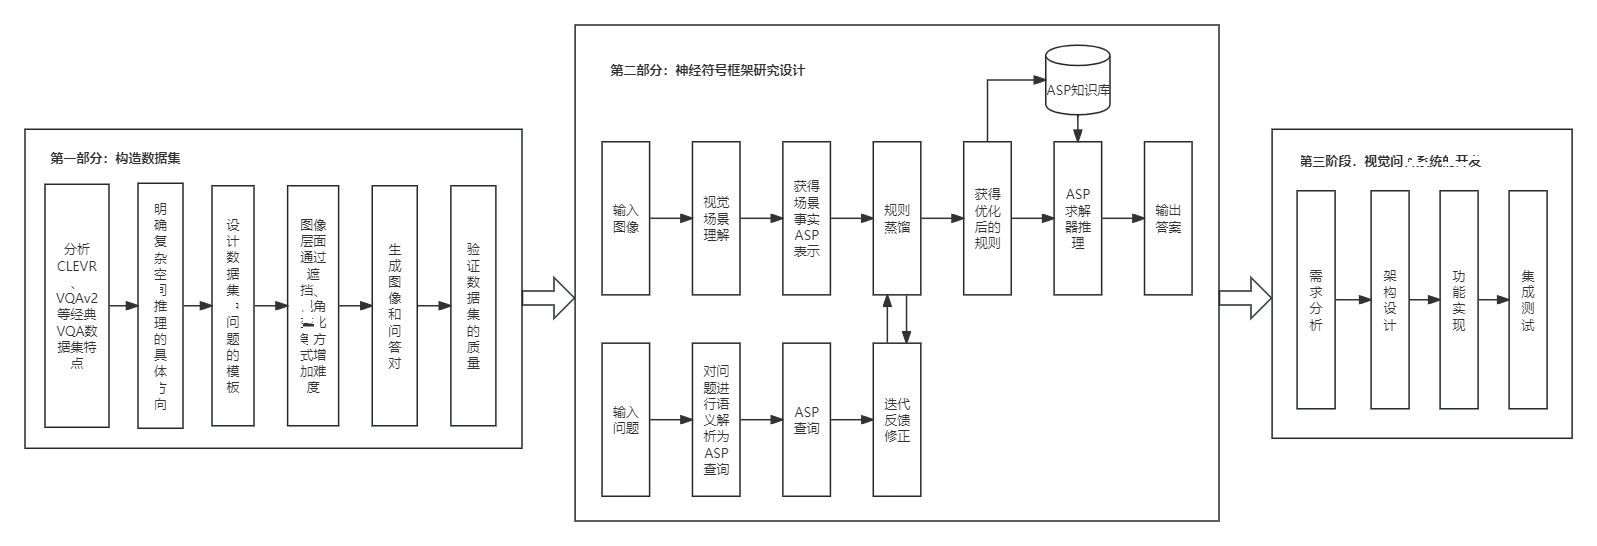
\includegraphics[width=\textwidth]{process.png}
    \caption{技术路线图\label{roadmap}}
\end{figure}

\section{论文结构}
本文共分为六个章节,各章节的主要内容具体如下:

第一章为绪论,总体介绍本文的研究背景及意义、相关研究现状与不足、研究目标
与研究内容、研究方法与技术路线及本文的结构安排。

第二章为背景知识,对本文涉及到的主要技术进行介绍,具体包括ASP程序语法及ASP求解器、
GLIP以及DSPy。

第三章为数据集构建。对本文所用的视觉问答数据集进行详细介绍,包括数据集的构造目的、数据集的研究方向、数据集的设计流程以及对数据集质量的验证。

第四章为神经符号框架的研究设计。对本文设计的神经符号框架进行详细介绍,包括流水线总体架构、视觉场景理解、语义解析、知识蒸馏、迭代反馈和规则修正、ASP推理等模块的设计。

第五章为实验及结果分析。通过一系列实验,验证本文所提出的神经符号框架对复杂空间推理任务的提升效果,以及其在不同大语言模型架构上的泛化能力。

第六章中对本文工作加以总结,分析本文的创新点和不足之处,并对未来的研究方向进行展望。
